\section{Precision-focused algorithms: Aggregation v.s. Retrieval Comparison}
% \subsection{Retrieval-based methods}
% This class of algorithms tries to identify good and bad workers, and then chooses the best worker segmentation as the output segmentation. In this paper, we look at two different ways of ranking workers and choosing the best worker. First, we use the {\em number of control points}, i.e. number of vertices in a worker's segmentation polygon to rank workers. This is a ranking scheme that~\cite{Vittayakorn2011} showed performs well in practice. Intuitively, workers that have used a larger number of points are likely to have been more precise, and provided a more complex and accurate segmentation. Other heuristic ranking scheme is described in more detail in our technical report~\cite{segmentation-tr}.
\begin{figure}[h!]
\vspace{-10pt}
\centering
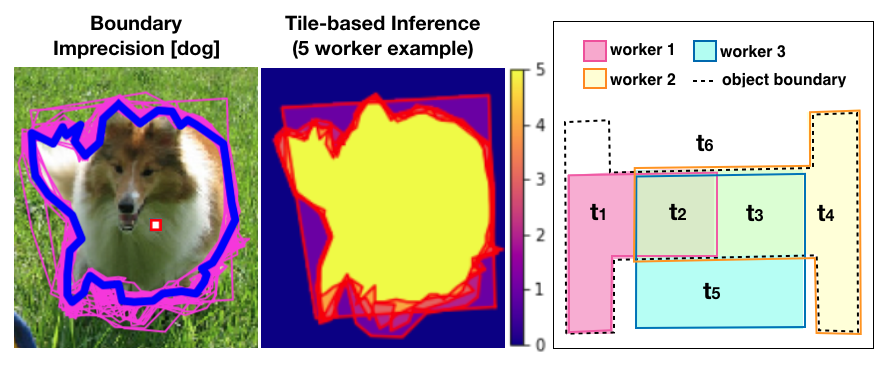
\includegraphics[width=0.8\textwidth]{plots/precision_issue_tile_example.png}
\caption{Left: Pink boundaries shows worker segmentations and blue delineates the ground truth. Right: Segmentation boundaries drawn by five workers shown in red. Overlaid segmentation creates a masks where the color indicates the number of workers who voted for the tile region.}
\label{tile_demo}
\end{figure}
\vspace{-10pt}
At the heart of our aggregation techniques is the ``tile'' data representation, where we logically overlay all workers' segmentations on top of each other, as illustrated in Figure \ref{tile_demo} right, to create non-overlapping discrete tile units. The intuition here is that by splitting the image into tiles, we get finer granularity information than by looking at complete segmentations. This also allows us to aggregate data from multiple workers rather than having to choose a single worker bounding box---enabling the opportunity to choose partial segmentations by fixing one worker's errors via the help from another worker's segmentation. Now, we will describe several algorithms for picking a good set of tiles.

\stitle{Aggregation: Majority Vote Aggregation (MV)} 
\par \noindent Include tiles in the output segmentation if and only if the tile is covered by at least 50\% of all worker segmentations.

\stitle{Aggregation: Expectation-Maximization (EM)}
\par \noindent Unlike MV, which assumes that all workers performs uniformly, EM approaches use worker quality models to infer the likelihood that a tile is part of the ground truth segmentation. The EM algorithm simultaneously estimate both worker qualities and tile likelihoods as hidden variables. Details of the formal derivation and three worker quality models that we have developed can be found in our technical report.

\stitle{Aggregation: Greedy Tile Picking (greedy)} 
\par \noindent Using tile probabilities from EM to estimate intersection area between ground truth and tile, then greedily pick tiles with the largest intersection area ratio until Jaccard score begins to decrease (effectively picking the largest and most probable tiles that should be included first). The Jaccard score is computed between the merged output from the selected set of tiles and MV segmentation.

\stitle{Retrieval: Number of Control Points (num pts)}
\par \noindent Pick the worker segmentation with the largest number of control points around the segmentation boundary (i.e. most precise drawing) as the output segmentation.

\subsection{Retrieval v.s. Aggregation-based Comparison}
 \begin{figure}[h!]
   \vspace{-10pt}
   \centering
   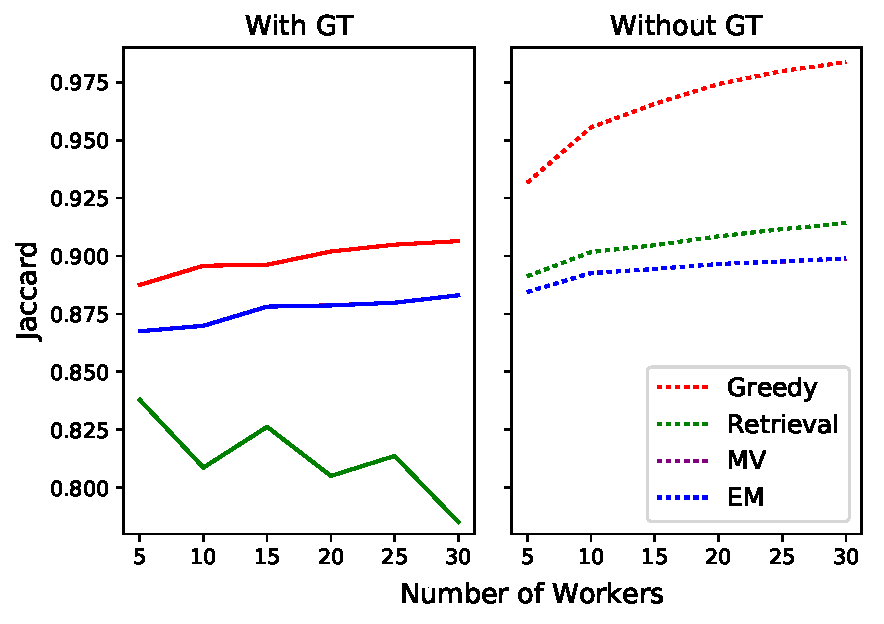
\includegraphics[width=0.9\textwidth]{plots/Retrieval_vs_Aggregation.pdf}
   \caption{Jaccard performance comparison between best-performing algorithms from retrieval and aggregation-based methods with clustering as a preprocessing step where possible. We compare between the original algorithms that do not make use of ground truth information (Left) and ones that do (Right). Note that MV and EM results are so close that they overlay on each other.}
   \label{retrieval_vs_aggregation}   
\end{figure} 
\vspace{-10pt}

\stitle{Aggregation-based methods performs significantly better than retrieval-based methods}
\par \noindent Figure~\ref{retrieval_vs_aggregation} left shows that amongst the algorithms that do not make use of ground truth information, the performance of aggregation-based algorithms (greedy, EM) exceeds the best achievable through the existing retrieval-based method (num pts). By making use of ground truth information (Figure~\ref{retrieval_vs_aggregation} right), the best aggregation-based algorithm can achieve a close-to-perfect average Jaccard score of 0.98 as an upper bound, far exceeding the results achievable by any single `best' worker (J=0.91). This result demonstrates that aggregation-based methods are able to achieve better performance by performing inference at the \textit{tile} granularity, which is guaranteed to be finer than any individual worker segmentation. 

\stitle{Performance of aggregation-based methods scales well as more workers segmentation are added.}
\par \noindent Intuitively, larger worker samples results in finer granularity tiles for the aggregation-based methods, resulting in an monotonically increasing relationship between number of worker segmentation used in the sample and performance evident in Table~\ref{statsTable}. However, worker scaling for retrieval-based methods are not guaranteed.
\begin{table}[h!]
   \small
     \setlength\tabcolsep{1.5pt}
      \begin{tabular}{l|l|l|l|l|l|l}
         & \multicolumn{2}{c|}{Retrieval-based} & \multicolumn{4}{l}{Aggregation-based} \\ \hline
      Algorithm         & num pts         & worker*        & MV    & EM    & greedy  & greedy*  \\ \hline
      Worker Scaling    & -6.30           & 2.58               & 1.63  & 1.64  & 2.16    & 5.59         \\ \hline
      Clustering Effect & 5.92            & -0.02              & 2.05  & 1.38  & 5.55    & -0.06       
      \end{tabular}
      \caption{The first row lists the average percentage change in Jaccard between 5 workers samples and 30 workers sample. The second row lists the average percentage change between the no clustering and clustering results. Algorithms with * makes use of ground truth information.}
      \label{statsTable}
\end{table}
\vspace{-10pt}

\stitle{Clustering as preprocessing improves algorithmic performance.}
\par \noindent Clustering results can also be used as a preprocessing step to any of the quality evaluation algorithms by keeping only the segmentations that belong to the largest cluster, which is typically free of any semantic errors. As shown in Table~\ref{statsTable}, on average, clustering generally results in an increase the resulting algorithmic performance. Since the ground-truth supervised variants are already free of semantic ambiguity and errors, there is minimal improvement resulting from clustering. %In particular, we see a greater improvement with clustering preprocessing for algorithms that are not very robust in resolving semantic errors or ambiguity, such as for the \texttt{num pts} retrieval algorithm, than compared to the aggregation-based methods. 